\documentclass[12pt,fleqn]{article}\usepackage{../common}
\begin{document}

\begin{minted}[fontsize=\footnotesize]{python}
import pandas as pd
df = pd.read_csv('oil2.csv',sep='\s*').T
print df.tail(10)
\end{minted}

\begin{verbatim}
             0
2004  83,160.1
2005  84,646.9
2006  84,631.1
2007  84,555.8
2008  85,719.3
2009  84,949.3
2010  87,524.9
2011  87,834.3
2012  89,700.3
2013  90,057.2
\end{verbatim}

$$ 
c = \frac{ 2c_m}{1 + \cosh |b_c(t-t_{mc})|   }
$$


\begin{minted}[fontsize=\footnotesize]{python}
from scipy.optimize import fmin
import pandas as pd
from numpy.linalg import *
df = pd.read_csv('oil1.csv',sep='\s*')

def hubbard(w):
    yfit = (2*w[0]) / (1+cosh( np.abs(w[1] * (df['year']-w[2])) ))
    diff = df['oil'] - yfit
    e=norm(diff)
    return e

v = fmin(hubbard, [2, 2, 1970], maxiter=100000, maxfun=10000)
print v
\end{minted}

\begin{verbatim}
Optimization terminated successfully.
         Current function value: 52.188303
         Iterations: 298
         Function evaluations: 540
[  8.38713684e+01  -4.77382480e-02   2.00814761e+03]
\end{verbatim}

\begin{minted}[fontsize=\footnotesize]{python}
df = df.set_index('year')
df['oil'].plot(oil)
plt.savefig('peak_01.png')
\end{minted}

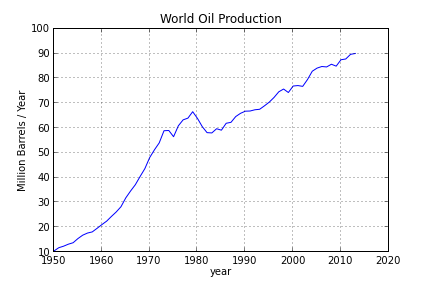
\includegraphics[height=6cm]{peak_01.png}

\url{http://www.earth-policy.org/Updates/2007/Update67_data2.htm#table1}

\url{http://en.wikipedia.org/wiki/Hubbert_curve}

\url{http://www.eia.gov/cfapps/ipdbproject/iedindex3.cfm?tid=5&pid=53&aid=1&cid=ww,&syid=1980&eyid=2013&unit=TBPD}

\url{http://www.countercurrents.org/mushalik270314.htm}


\end{document}
